% This document is used for Daya Bay MACRO PMT pressure test report


\documentclass{beamer}
\usepackage{graphicx}

\newcommand{\tabincell}[2]{\begin{tabular}{@{}#1@{}}#2\end{tabular}}

\usepackage{ragged2e}
\justifying

\usepackage{setspace}

\setbeamertemplate{navigation symbols}{}
\setbeamertemplate{footline}[page number]
\setbeamertemplate{caption}[numbered]

\usetheme{default}
\logo{
\includegraphics[height=1cm]{Dyb_logo.png}}
\begin{document}
\title{Status of MACRO \& Hamamatsu PMT pressure tests at SAB}
\author{Logan Lebanowski, Shih-Kai Lin}
\institute{University of Houston}
\date{2010 November 4}

\begin{frame}
\begin{center}
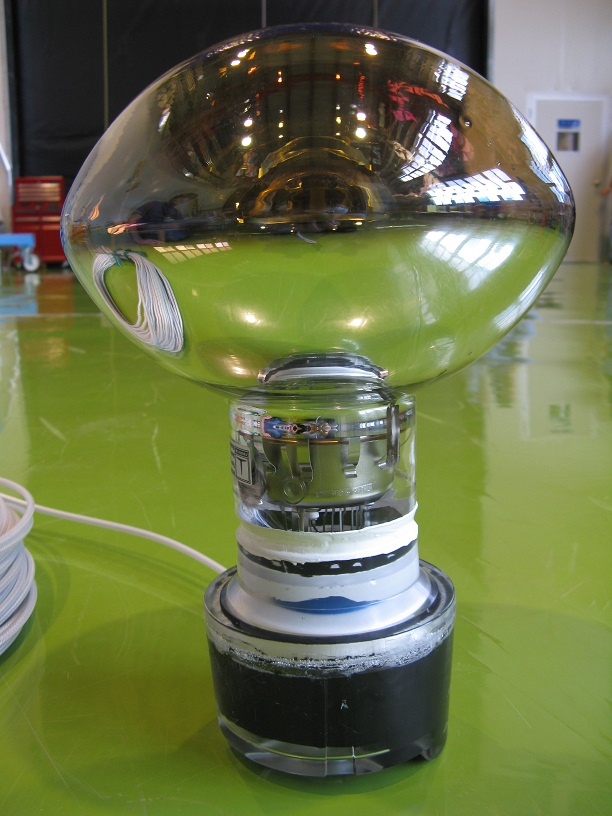
\includegraphics[height=4cm]{IMG_1048.jpg}
\end{center}
\titlepage
\end{frame}


\begin{frame}{overview}
	\begin{itemize}
		\item 150 waterproof MACRO EMI PMT assemblies as well as 16
			Hamamatsu waterproof PMTs need to be pressure tested
			at the SAB. They have already passed performance tests at DGUT.
		\item We test about 10 PMTs per week (mid-August to December).
		\item For more information, see
			\textcolor{blue}{\href
			{http://dayabay.ihep.ac.cn/cgi-bin/DocDB/ShowDocument?docid=5373}{doc 5373}}.
	\end{itemize}
		\begin{center}
			\underline{As of November 4, we have passed 77 of 86 tested MACRO PMTs}\\
			\underline{and 16 of 16 tested Hamamatsu PMTs.}
		\end{center}
	\begin{center}
		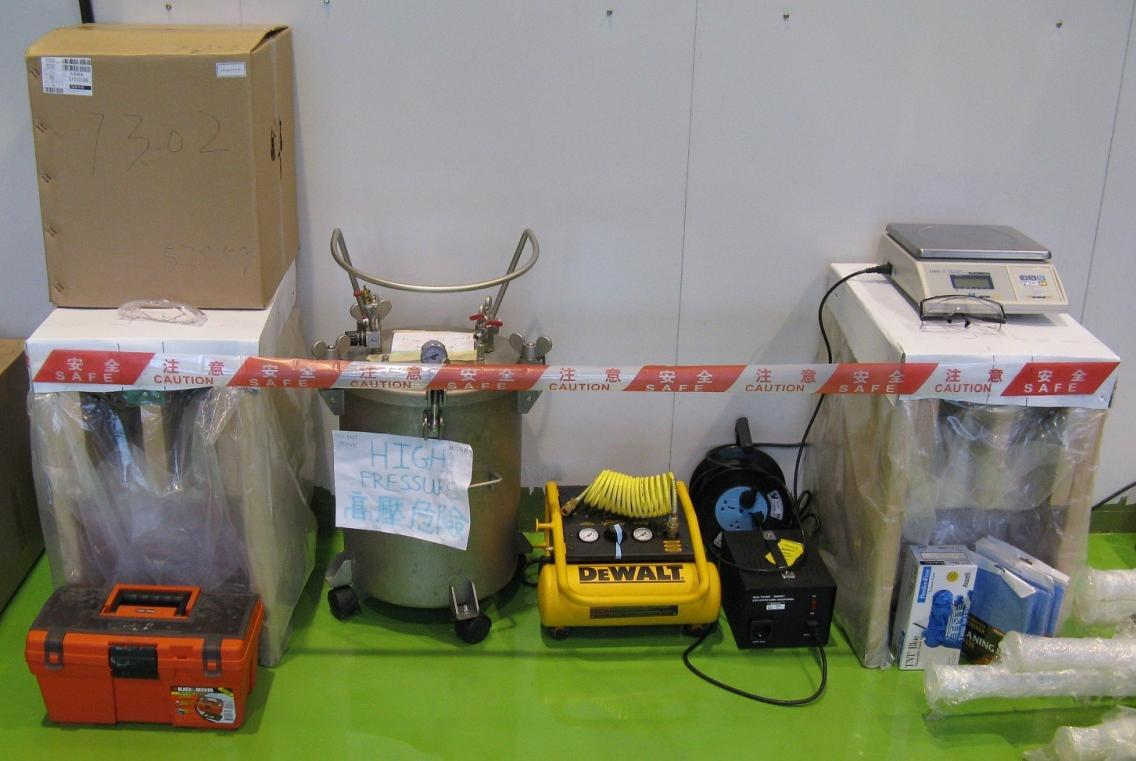
\includegraphics[height=4cm]{test_setup.jpeg}
	\end{center}
\end{frame}


\begin{frame}{pressure test results}
	\begin{center}
		\small
		11 PMTs were tested during the past week (October 28 - November 3).
	\end{center}
\begin{table}
\small
\setstretch{0.4}
\begin{tabular}{c|c|c|c|c}
%\setlength{\tabcolsep}{2pt}
	SN$^\dagger$ & mass$^\ddag$(g) & pressure (psig) & test time (h:m) & result \\
	\hline
	WSD2719 & 4525.5 & 20.1 & 14:45 & PASS$^1$ \\

	WSD2722 & 4550.5 & 20.1 & 8:23 & PASS$^1$ \\

	WSD2692 & 4557.5 & 20.1 & 14:47 & PASS$^1$ \\

	WSD2607 & 4560.0 & 20.1 & 7:45 & PASS$^1$ \\

	8589 & 564.5 & 12.2 & 15:17 & PASS$^2$ \\

	6346 & 636.5 & 12.0 & 47:52 & PASS$^2$ \\

	7196 & 596.0 & 12.0 & 8:35 & PASS$^2$ \\

	7031 & 578.0 & 12.0 & 15:39 & PASS$^3$ \\

	6287 & 663.0 & 12.0 & 7:54 & PASS$^2$ \\

	8377 & 588.5 & 12.0 & 15:01 & NOT PASS$^4$ \\

	6280 & 654.0 & 12.1 & 8:01 & PASS$^2$ \\

\end{tabular}
%\caption {pressure test result: For PASS/FAIL reasons, please see the table in the next slide.}
\end{table}
	\setstretch{0.1}
	\tiny
	$^\dagger$ Serinal numbers with(without) ``WSD'' prefix are Hamamatsu(MACRO) waterproof PMTs. \\
	$^\ddag$ For MACRO PMTs, this means unpotted weight. For Hamamatsu PMTs, this is the total
			weight of PMT+cable.\\
	$^1$ Cable dry. No cracks. No leaks detected by weighing before and after testing
		(see the last page.)\\
	$^2$ Cable dry. No leaks or cracks.\\
	$^3$ 2+Some water penetrated the mastic tape seal of the cable
		strain relief plug, but did not penetrate the UW cable plug.\\
	$^4$ Cable end sealing tube was full of water. It will be fixed and tested again.

%\begin{itemize}
%	\item For PASS/FAIL reasons, please see the table in the next slide.
%\end{itemize}
%	\setlength{\tabcolsep}{2pt}
%	\tiny
%	\begin{table}
%		\begin{tabular}{|c|p{3.5in}|}
%		\hline
%		1 & Cable dry. No cracks. No leaks detected to within 3.0g
%		    (determined by weighing before and after testing.)\\
%		\hline
%		3 & Cable sealing tube still had some water. The way the cable was repaired didn't
%		work well.\\
%		\hline
%		\end{tabular}
	%\caption{PASS/FAIL reasons}
%	\end{table}
\end{frame}

\begin{frame}{signal test results}
	\setstretch{0.3}
	\small The operational capability of a PMT is verified after pressure testing:\\
	{\scriptsize The PMT is placed in a dark box, connected to a single channel decoupler box,
	and set to its 2E7 gain voltage, as recorded in the DGUT data. After tens of minutes,
	the count rate, rise time, and pulse height are recorded. We use a threshold of 3.00 
	mV, which is roughly 1/4 pe.
	}

	\setstretch{1}
	\setlength{\tabcolsep}{2pt}
	\small
	\begin{center}
	\begin{tabular}{|l|p{1.2cm}|p{1.9cm}|p{1.5cm}|p{1.7cm}|}
		\hline
		\textbf{SN}$^\dagger$&\textbf{Rate (kHz)}&\textbf{DGUT rate (kHz)}&\textbf{Rise time (ns)}&
		\textbf{DGUT rise time (ns)}\\
		\hline
		\hline
		7487   &1.3&0.39&5.0&6.0\\
		7508   &8.0&0.36&5.0&6.8\\
		WSD2592&3.2&2.0&3.2&4.37\\
		WSD2717&5.5&1.64&3.2&4.28\\
		WSD2606&6.0&1.5&3.2&3.23\\
		WSD2605&5.5&1.22&3.2&4.15\\
		WSD2614&3.5&0.94&3.4&3.75\\
		WSD2719&12.0&1.42&3.2&4.212\\
		WSD2722&2.2&1.56&3.2&3.634\\
		WSD2692&3.0&1.22&3.1&3.782\\
		WSD2607&3.5&1.08&3.2&4.44\\
		\hline
	\end{tabular}
	\tiny
	\\$^\dagger$ Serinal numbers with(without) ``WSD'' prefix are Hamamatsu(MACRO) waterproof PMTs. \\
		\begin{itemize}
			\tiny
			\item Rates are all below 10 kHz but in 1 case. It could be below 10 kHz if it
			was given enough time.
		\end{itemize}
	\end{center}
\end{frame}

\begin{frame}{summary}
	\begin{itemize}
		\item We finished testing a sample of 16 Hamamatsu waterproof PMT assemblies at SAB.
		All pressure and signal tests were passed:
		\begin{itemize}
			\item No leaks were detected by weighing before and after pressure testing.
			Actually, the Hamamatsu PMTs were always lighter by $\sim$1.5 g (dirt removed?).
			\item Hamamatsu PMTs' dark rates begin at lower initial values than MACROs
			and they have shorter rise times and larger pulse heights.
		\end{itemize}
		\item 64 MACRO PMTs remain to be tested. At 10 per week, we should finish by Christmas.
	\end{itemize}
\end{frame}


\end{document}

